\chapter{无线与移动网络}

\noindent\textbf{本章要解决的问题。} 有线网络中的主机通常通过固定链路接入；无线网络则让主机借助无线电链路通信，但信号会衰减、受干扰，还可能在接收端发生发送者彼此听不到的冲突。移动网络还要解决另一个问题：设备改变接入点或运营商网络后，数据怎样继续找到它。本章依课件顺序学习无线网络概述、无线链路特性、IEEE 802.11 无线局域网、蜂窝网络结构、网络移动管理、移动 IP、蜂窝网切换以及无线对高层协议的影响。

\section{无线与移动网络概述}
\subsection{无线与移动是两个不同概念}
\textbf{无线}表示通信链路使用无线电等非有线介质；\textbf{移动}表示设备在网络接入点之间移动时，网络仍要处理其位置变化。一个设备可以是无线但静止的，例如固定安装的无线传感器；也可以移动但暂时关闭无线通信。因此“无线网络”和“移动网络”关注的挑战不同：前者要解决无线链路上的传输和共享问题，后者要解决接入点改变后如何维持连接与寻址。

\textbf{无线主机}是运行应用程序并通过无线链路收发数据的终端，例如笔记本电脑、智能手机和物联网设备。\textbf{基站}通常连接到有线网络，在其覆盖范围内中继无线主机与有线网络之间的数据；蜂窝网络中的基站和 Wi-Fi 中的接入点都承担类似角色。\textbf{无线链路}可以连接主机与基站，也可以连接网络中的其他节点；多个主机共享链路时，需要多路访问控制协议协调谁在何时发送。

\subsection{无线网络的两种组织方式}
\textbf{基础设施模式}中，无线主机先连接基站，再由基站接入更大的有线网络。无线主机从一个基站换到另一个基站称为\textbf{切换}（handoff/handover）；切换期间网络需要更新接入关系。\textbf{特定网模式}（ad hoc，自组网）没有预先部署的基站，节点自行组织网络；若目的节点不在直接无线覆盖范围内，中间节点还要转发数据，兼任终端和路由节点。

课件还用两个维度分类无线网络：是否有基础设施、通信需经过几跳。基础设施单跳网络如普通 Wi-Fi，主机经接入点（AP，Access Point）接入互联网；无基础设施单跳网络如近距离点对点连接；多跳网络让数据经过多个无线节点中继。基础设施多跳网络可形成无线网状网络；无基础设施多跳网络包括移动自组网（MANET，Mobile Ad Hoc Network）和车载自组网（VANET，Vehicular Ad Hoc Network）。这些名称描述网络组织方式，不代表所有这类网络必然具有同一套路由协议。

课件以 2019 年的用户与宽带连接比例说明无线接入的重要性。这些数字是课件所用的历史背景数据，不应当作当前统计值。参考教材把无线归入传输介质和局域网等章节，本节的网络分类、结构图以课件为主。
\annotationarea[4]
\small 来源：课件 \texttt{Chapter7-无线与移动网络.pdf}，PDF阅读器第4--12页（对应显示页4--12）；无线介质概念参考《2027年计算机网络考研复习指导》第2章§2.2.1，PDF第53--55页（印刷第42--44页）。\normalsize

\section{无线链路与网络特性}
\subsection{衰减、干扰与多径传播}
无线电波在传播过程中能量会随距离和环境减弱，这称为\textbf{路径损耗}。障碍物、墙体和距离变化都会让接收信号强度改变。多个设备可能使用相同或相邻频段，产生\textbf{干扰}。无线信号还可能被墙壁、地面或物体反射，沿不同路径、在不同时间到达接收端，这称为\textbf{多径传播}。多条路径上的信号叠加后可能增强，也可能互相抵消，因而接收质量会随位置和时间变化。

\textbf{信噪比}（SNR，Signal-to-Noise Ratio）描述有用信号相对于噪声的强弱；信噪比越高，通常越容易从噪声中恢复信号。\textbf{误码率}（BER，Bit Error Rate）是传输中错误比特占总比特的比例。给定物理层方案时，提高发射功率通常能提高 SNR、降低 BER；给定 SNR 时，调制方式越复杂通常能承载更高速率，但要满足更低的误码要求。设备会根据链路质量调整调制方式和速率：链路变差时改用较低速率以降低误码，链路变好时再尝试较高速率。

\subsection{隐藏终端与信号衰减}
无线节点的可侦听范围和接收端的覆盖范围不一定相同。\textbf{隐藏终端问题}是指两个发送端彼此听不到，却都能到达同一个接收端。例如 A 和 C 都能与 B 通信，但 A、C 互相听不到；二者若同时给 B 发送，信号会在 B 处冲突。\textbf{信号衰减导致的冲突}也会产生相同后果：A、C 的信号分别足以到达 B，但在对方所在位置已经弱到无法侦听，于是它们误以为信道空闲。

\begin{figure}[H]\centering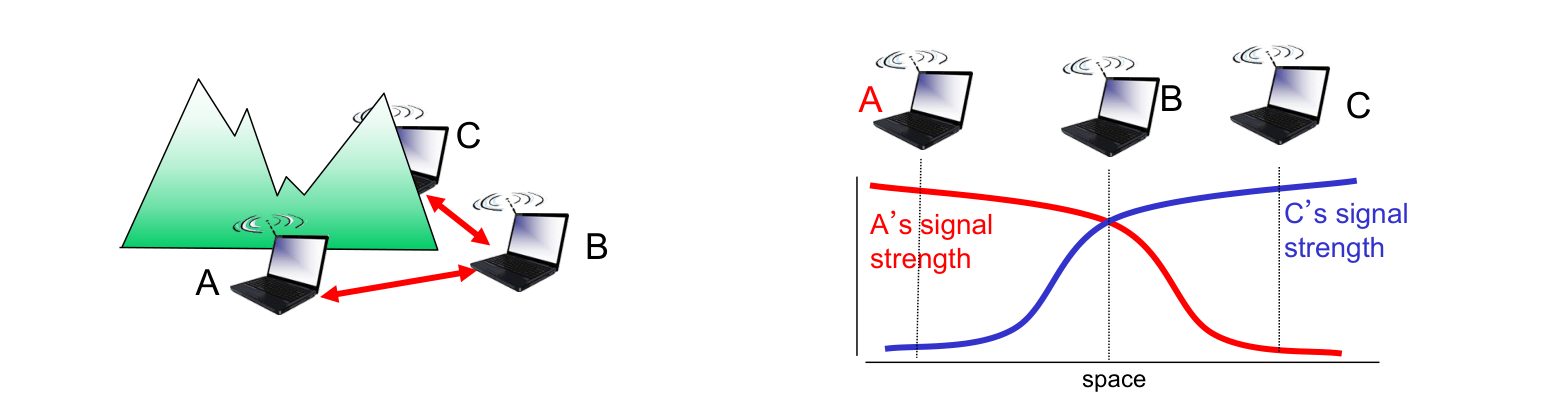
\includegraphics[width=.91\textwidth]{ch07-hidden-terminal.png}\caption{隐藏终端与信号衰减示意：A、C 各自能到达 B，却无法互相侦听；右侧曲线表示两发送端信号强度随位置变化。来源：\texttt{Chapter7-无线与移动网络.pdf}，PDF阅读器第16页（显示页16），局部截取。}\label{fig:ch07-hidden-terminal}\end{figure}

这说明无线节点只监听自己位置的信道，不能保证知道接收端是否会发生冲突；无线网卡也难以像有线以太网那样边发送边检测所有冲突。IEEE 802.11 因而采用冲突避免和确认重传机制，尽量减少冲突并判断帧是否成功到达。
\annotationarea[4]
\small 来源：课件PDF阅读器第14--16页（显示页14--16）；参考教材第3章§3.6.3，PDF第104--107页（印刷第93--96页），用于核对无线信道、隐藏站与CSMA/CA机制。\normalsize

\section{无线局域网：802.11 标准}
\subsection{802.11 标准与基本服务集}
IEEE（Institute of Electrical and Electronics Engineers，电气电子工程师学会）802.11 是无线局域网标准族，常见产品通常称 Wi-Fi。不同版本在频段、物理层技术和最高数据率方面不同。\textbf{直接序列扩频}（DSSS，Direct Sequence Spread Spectrum）把数据扩展到较宽的码片序列；\textbf{正交频分复用}（OFDM，Orthogonal Frequency Division Multiplexing）把数据并行映射到相互正交的多个子载波；\textbf{多输入多输出}（MIMO，Multiple-Input Multiple-Output）使用多根发射、接收天线提高传输能力。表中数据是课件列出的速率和距离，实际速率与覆盖范围会受设备、信道带宽、干扰及环境影响。

\begin{center}\small
\begin{tabularx}{.98\textwidth}{l l l X}\toprule
课件列出的版本 & 频段 & 最高速率 / 距离（课件值） & 课件强调的物理层特点 \\\midrule
802.11b & 2.4--2.5 GHz & 11 Mb/s / 约30 m & DSSS；课件称成本低、传播距离较远 \\
802.11a & 5--6 GHz & 54 Mb/s / 约30 m & OFDM；速率较高、覆盖相对短 \\
802.11g & 2.4--2.5 GHz & 54 Mb/s / 约30 m & OFDM \\
802.11n（Wi-Fi 4） & 2.4/5 GHz & 600 Mb/s / 约70 m & MIMO 与 OFDM；课件提到40 MHz带宽 \\
802.11ac（Wi-Fi 5） & 5 GHz & 约3.47 Gb/s / 约70 m & 课件表列值 \\
802.11ax（Wi-Fi 6） & 2.4/5 GHz & 约14 Gb/s / 约70 m & 课件表列值 \\
802.11af / ah & 54--790 MHz / 约900 MHz & 35--560 / 347 Mb/s；约1 km & 课件强调较远距离 \\\bottomrule
\end{tabularx}\end{center}

课件第18页对 802.11b/a/g/n 还列出了最高数据率及频段；第20页扩展了版本和距离表。表内“2020（exp.）”等年代与速率应理解为课件资料的记录时点，不用于推断今天的部署情况。课件称这些 Wi-Fi 网络既可工作于基础设施模式，也可工作于自组网模式，并采用 CSMA/CA（Carrier Sense Multiple Access with Collision Avoidance，载波监听多路访问/冲突避免）进行多路访问。802.11b 的课件说明还指出同一网络中的主机使用相同的扩频码片序列。

基础设施模式中的基站称为\textbf{接入点}（AP，Access Point）。一个\textbf{基本服务集}（BSS，Basic Service Set）是一个 AP 及与它通信的无线主机所组成的局部网络，课件也称其为一个 cell。主机要先选择并关联到 AP，之后才能通过该 AP 接入更大的网络。课件还画出没有 AP、只有主机组成的 ad hoc 网络。

\subsection{信道选择、扫描与关联}
无线频谱被分成不同信道，AP 选择信道工作；相邻 AP 若选用相同或相邻信道，可能互相干扰。主机通过扫描发现 AP：AP 的信标帧（beacon）包含网络名称\textbf{服务集标识符}（SSID，Service Set Identifier）及 AP 的 MAC 地址。主机选定 AP 后发起关联；网络可能还要进行身份认证。成功接入局域网后，主机通常通过\textbf{动态主机配置协议}（DHCP，Dynamic Host Configuration Protocol）获得 IP 地址等配置。

课件区分两种扫描过程：\textbf{被动扫描}中，各 AP 周期性发送信标，主机监听并选择 AP，再发送关联请求，AP 返回关联响应；\textbf{主动扫描}中，主机先广播探测请求（Probe Request），AP 回探测响应（Probe Response），之后主机发送关联请求、AP 返回关联响应。两种方式都是先发现候选 AP，再完成关联；主动扫描多出探测请求/响应这一对报文。

\begin{figure}[H]\centering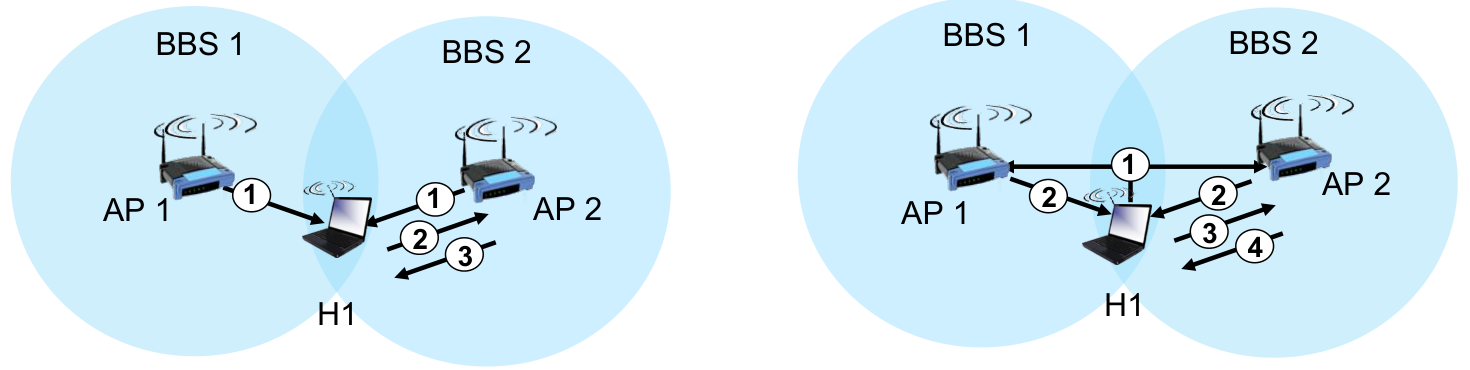
\includegraphics[width=.93\textwidth]{ch07-wifi-scan.png}\caption{被动与主动扫描：左边 AP 主动发送信标，右边主机先发 Probe Request；圆圈编号表示报文事件次序。来源：\texttt{Chapter7-无线与移动网络.pdf}，PDF阅读器第23页（显示页23），局部截取。}\label{fig:ch07-wifi-scan}\end{figure}
\annotationarea[4]

\subsection{CSMA/CA 与 RTS/CTS 信道预约}
CSMA（Carrier Sense Multiple Access，载波监听多路访问）要求发送前先监听信道。有线以太网的 CSMA/CD（Carrier Sense Multiple Access with Collision Detection，载波监听多路访问/冲突检测）可以在发送时检测碰撞并停止发送；802.11 无线网很难在强发送信号旁检测微弱接收信号，而且隐藏终端使发送端看不到接收端处的所有碰撞，因此使用 CSMA/CA（Carrier Sense Multiple Access with Collision Avoidance，载波监听多路访问/冲突避免）。“避免”是降低冲突概率，不保证冲突绝不发生。

课件描述的发送端规则如下：
\begin{enumerate}[nosep]
  \item 若信道空闲持续一个 DIFS（Distributed Inter-Frame Space，分布式协调帧间间隔）时间，发送整个帧。发送过程中不做冲突检测。
  \item 若信道忙，或上次未收到确认，选取随机退避时间。信道空闲时退避计时器递减；信道变忙时计时器暂停，等重新空闲后再继续。
  \item 计时器到零时发送帧。接收方正确收到帧后，等待更短的 SIFS（Short Inter-Frame Space，短帧间间隔）再回 ACK（Acknowledgment，确认帧）。SIFS 短于 DIFS，使当前数据交换中的 ACK 优先于新的竞争发送。
  \item 若发送端没有收到 ACK，就认为帧可能丢失或冲突，扩大随机退避间隔后重试。
\end{enumerate}

\begin{figure}[H]\centering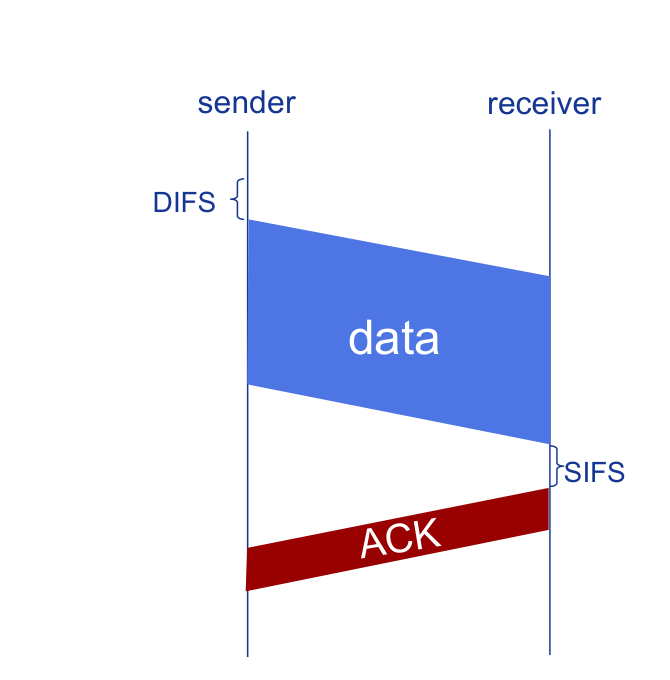
\includegraphics[width=.56\textwidth]{ch07-csma-ca-timing.png}\caption{CSMA/CA 发送时序：发送端等待 DIFS 后发送数据，接收端再等待 SIFS 并回 ACK。图中横向为时间，纵向两条线分别表示发送端和接收端。来源：\texttt{Chapter7-无线与移动网络.pdf}，PDF阅读器第25页（显示页25），局部截取。}\label{fig:ch07-csma-ca-timing}\end{figure}

当隐藏终端较明显时，可用请求发送帧 RTS（Request To Send）和允许发送帧 CTS（Clear To Send）预约信道。发送端先按 CSMA 规则竞争并发送 RTS；接入点正确收到后，经 SIFS 返回 CTS。周围节点能听到 CTS 后会推迟发送，随后发送端经 SIFS 发送数据，接收端再经 SIFS 返回 ACK。RTS 本身仍可能冲突，但它短于数据帧，因此冲突造成的浪费较小。RTS/CTS 是可选的预约办法，不表示无线冲突从此完全消失。

\textbf{网络分配向量}（NAV，Network Allocation Vector）是节点根据帧中的 Duration（持续期）字段设置的虚拟忙碌计时器。即使节点没有听到隐藏发送端的 RTS，只要它听到接入点发出的 CTS，就能从持续期字段知道应暂缓发送多久。物理载波监听是实际检测无线信号；NAV 是按收到的预约通知推算信道将被占用的时间。

\begin{figure}[H]\centering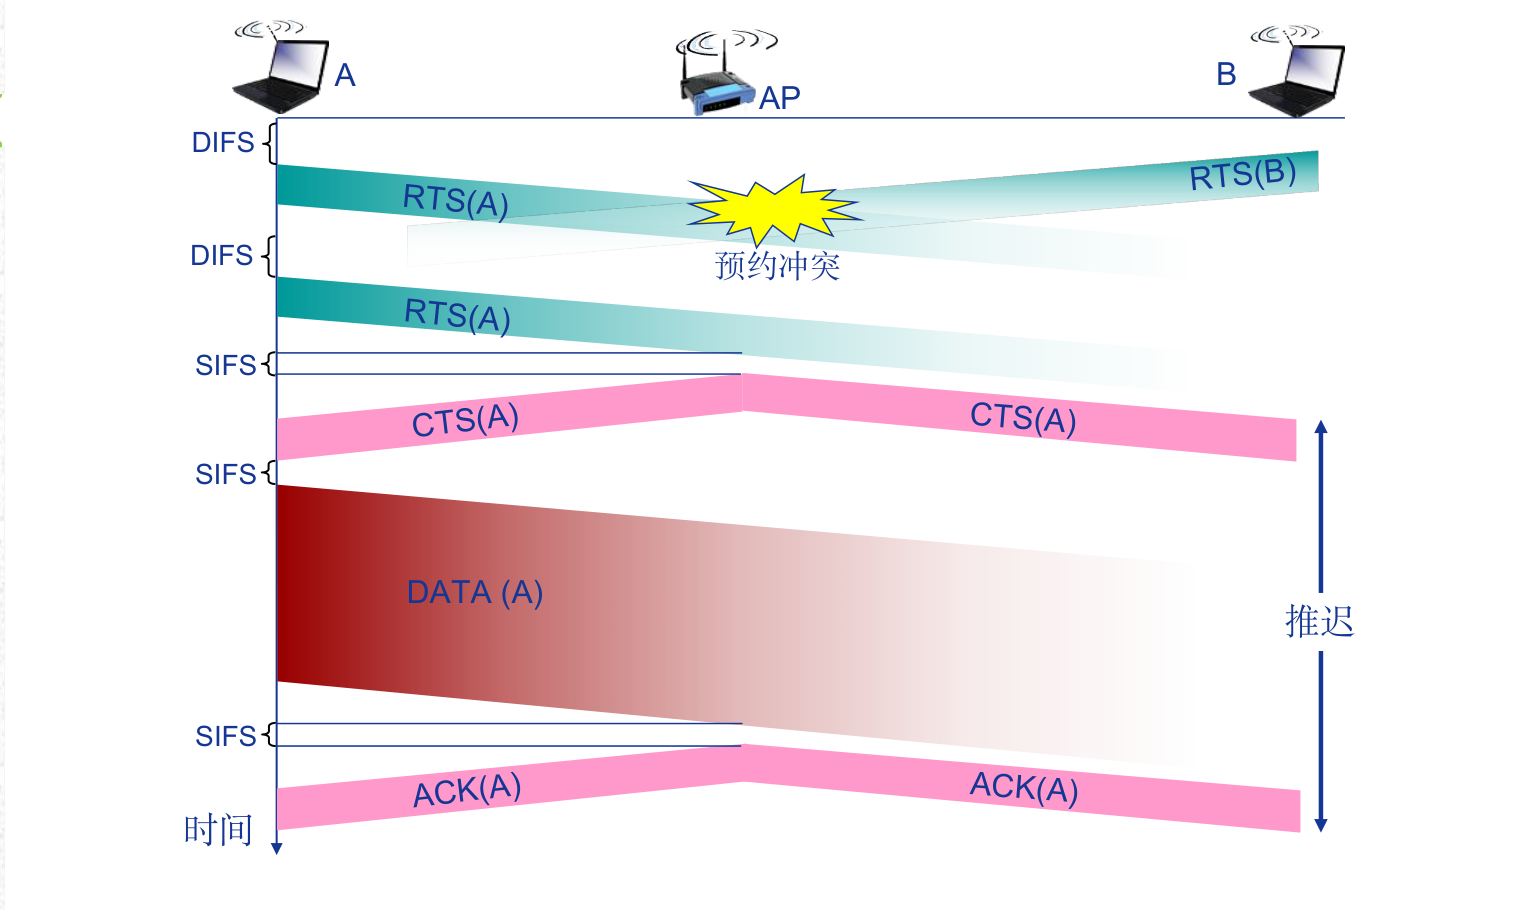
\includegraphics[width=.91\textwidth]{ch07-rts-cts.png}\caption{RTS/CTS 预约时间线：A 与 B 的 RTS 可发生冲突；接入点收到 A 的 RTS 后回 CTS，B 听到 CTS 后推迟，A 再发送 DATA 并收到 ACK。横向箭头为时间，纵向为不同节点。来源：\texttt{Chapter7-无线与移动网络.pdf}，PDF阅读器第27页（显示页27），局部截取。}\label{fig:ch07-rts-cts}\end{figure}

\textbf{课件例题（PDF第28页）：} 忽略传播、处理及所有帧的发送时间，某主机从希望发送开始，到收到接收正确的确认帧，最快需要多久？假设信道空闲且不需要随机退避。

\textbf{解：} 从希望发送到收到确认，按事件顺序是：发送端先等待 DIFS，再发 RTS；接收端收到 RTS 后等待第一个 SIFS，再回 CTS；发送端收到 CTS 后等待第二个 SIFS，再发 DATA；接收端收到 DATA 后等待第三个 SIFS，再回 ACK。题目让忽略 RTS、CTS、DATA、ACK 的发送时间，以及传播和处理时间，所以只把帧间等待相加：第一个控制帧前的 DIFS，加上 RTS--CTS、CTS--DATA、DATA--ACK 三个相邻帧间的 SIFS。
\[
  T_{\min}=\mathrm{DIFS}+3\,\mathrm{SIFS}.
\]
若信道一开始忙或产生冲突，就还要加上推迟接入和随机退避时间；题目所给假设排除了这些等待。
\annotationarea[4]
\small 来源：课件PDF阅读器第24--28页（显示页24--28）；参考教材第3章§3.6.3，PDF第105--107页（印刷第94--96页），核对DIFS/SIFS、随机退避、ACK、NAV及RTS/CTS过程。\normalsize

\subsection{802.11 MAC 帧及地址字段}
MAC（媒体访问控制，Medium Access Control）帧负责在本地链路上传送数据。课件给出的 802.11 帧结构包含：帧控制字段2字节、持续期2字节、地址1至3（各6字节）、序号控制2字节、可选地址4（6字节）、载荷0--2312字节以及 CRC（Cyclic Redundancy Check，循环冗余校验）4字节。帧控制字段里含协议版本、帧类型/子类型，以及“去往AP”“来自AP”、重试等标志；RTS、CTS、ACK 和数据帧由类型/子类型区分。持续期字段供信道预约使用，序号字段帮助识别帧和重传。

四个地址的含义取决于帧是否“去往 AP”以及是否“来自 AP”。在基础设施模式下，直接无线接收方/发送方与原始数据报的最终目的/原始来源可能不同，所以地址字段需要同时记录无线跳的两端和端到端的源/目的。DA（Destination Address）表示最终目的地址，SA（Source Address）表示原始源地址，BSSID（Basic Service Set Identifier）表示该基本服务集的标识地址；RA（Receiver Address）/TA（Transmitter Address）分别表示当前无线链路上的接收方/发送方。IBSS 表示 Independent Basic Service Set（独立基本服务集）；WDS 表示 Wireless Distribution System（无线分布系统）。

\begin{center}\small
\begin{tabularx}{.98\textwidth}{l c c X X X X}\toprule
场景 & 去往AP & 来自AP & 地址1 & 地址2 & 地址3 & 地址4 \\\midrule
IBSS（无基础设施） & 0 & 0 & DA & SA & BSSID & — \\
主机发往AP & 1 & 0 & AP/BSSID（RA） & 主机SA（TA） & 最终DA & — \\
AP发往主机 & 0 & 1 & 主机DA（RA） & AP/BSSID（TA） & 原始SA & — \\
WDS（无线分布系统） & 1 & 1 & RA & TA & DA & SA \\\bottomrule
\end{tabularx}\end{center}

\textbf{逐步读例：} 主机 H1 向同一局域网中的路由器 R 发送时，无线帧当前直接发给 AP，所以“去往AP=1、来自AP=0”：地址1是 AP 的 MAC，地址2是 H1 的 MAC，地址3是最终目的 R 的 MAC。AP 把数据转成有线以太网帧时，源 MAC 是 H1、目的 MAC 是 R。反向由 AP 发给 H1 时，“去往AP=0、来自AP=1”：地址1为 H1，地址2为 AP，地址3保留原始源地址。

\begin{figure}[H]\centering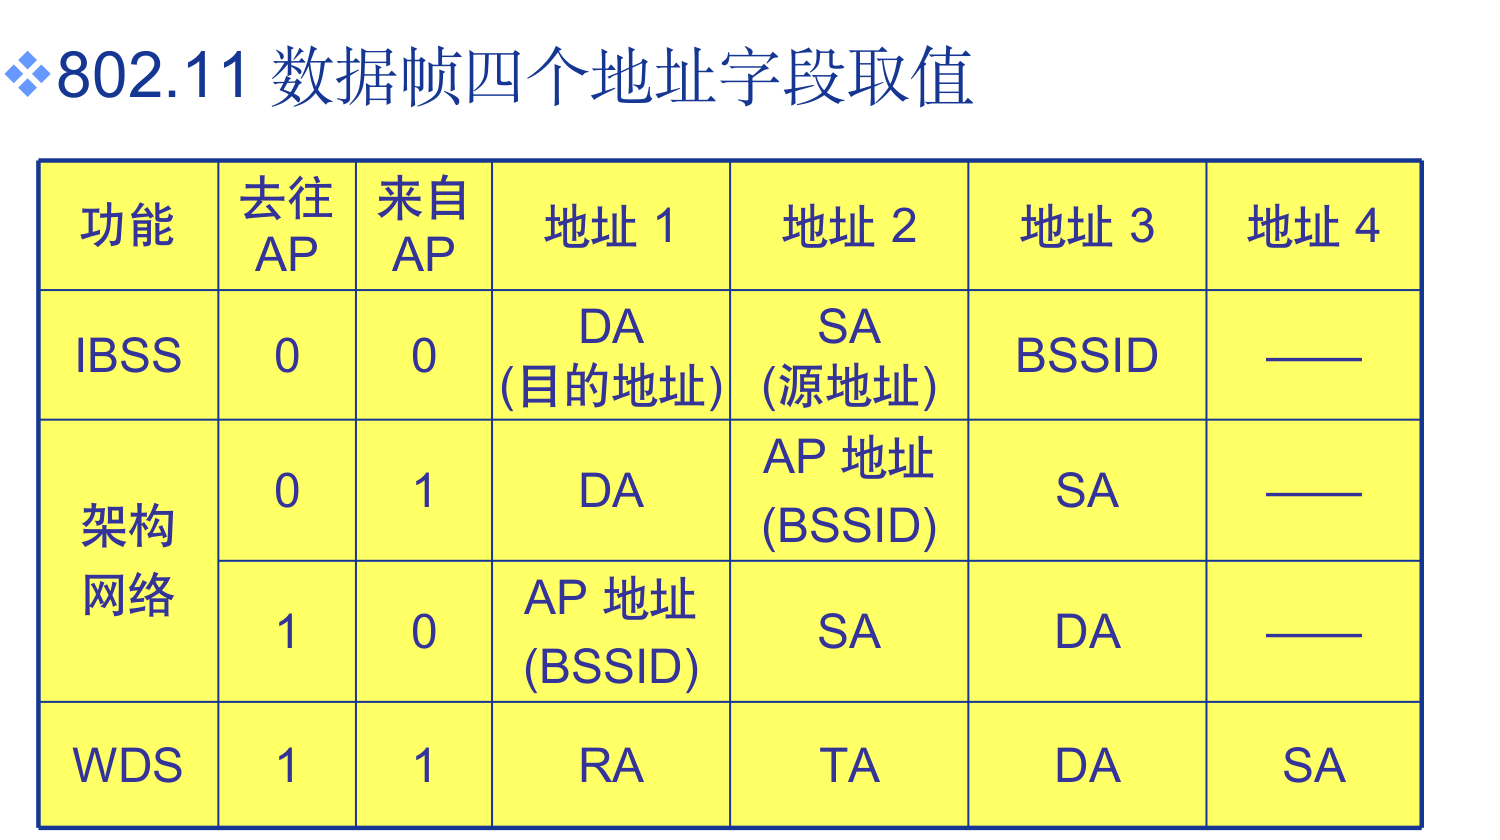
\includegraphics[width=.9\textwidth]{ch07-wifi-addresses.png}\caption{课件列出的四地址取值表。先读“去往AP/来自AP”两位，再按表确定地址1--4；WDS 行使用四个地址。来源：\texttt{Chapter7-无线与移动网络.pdf}，PDF阅读器第32页（显示页32），局部截取。}\label{fig:ch07-wifi-addresses}\end{figure}

\textbf{课件两页的表述不一致：} 第30页文字称地址4用于 ad hoc 或无线桥接；第32页表格则将 IBSS（自组网，去往/来自 AP 均为0）列为地址4空缺，只在 WDS（两位均为1）列出地址4。上述规则按课件第32页的完整取值表整理；复习时应注意第30页这句与表格之间的差异。
\annotationarea[4]
\small 来源：课件PDF阅读器第29--33页（显示页29--33）；参考教材第3章§3.6.3，PDF第108--109页（印刷第97--98页）。课件第30页关于地址4的描述与第32页取值表不一致，已在正文标明。\normalsize

\subsection{同子网移动、速率适应与节电}
如果主机在同一个互联网协议（IP，Internet Protocol）子网内从一个 AP 移动到另一个 AP，IP 地址可以保持不变。交换机通过主机发出的帧学习“该主机媒体访问控制（MAC，Medium Access Control）地址从哪个端口到达”，从而更新到达主机的端口信息。接入点改变是链路层位置变化，不必然意味着网络层 IP 地址改变。

无线信道质量变化时，设备还可以做\textbf{速率适应}：远离基站时 SNR 下降、BER 上升；当误码过高，就切换到较低速率的物理层方案，使传输更可靠。无线设备会在吞吐率与误码风险之间作选择。

\textbf{功率管理}用于节约电池。Wi-Fi 主机可通知 AP 自己进入休眠，AP 暂不向它发送帧并缓存下行数据；主机在下一个信标之前醒来。信标中的待发列表若显示 AP 有缓存帧，主机保持唤醒并接收；若无待发帧则继续休眠。

\subsection{蓝牙个人区域网络}
课件用蓝牙说明短距离无线个人区域网（PAN，Personal Area Network）。蓝牙覆盖范围通常小于10米，用于替代鼠标、键盘、耳机等设备的短连接；课件所列传统蓝牙使用2.4--2.5 GHz ISM（Industrial, Scientific and Medical，工业、科学和医疗）频段，速率最高约3 Mb/s。它可在没有固定基础设施时组织成微微网（piconet）：一个主控设备轮询客户端，为客户端传输请求分配机会。课件还介绍每个时隙约625微秒，并按已知伪随机次序在79个频率信道间跳频；停泊（parked）状态让暂不活动的设备休眠以节电。

\annotationarea[4]
\small 来源：课件PDF阅读器第34--38页（显示页34--38）；参考教材第3章§3.6.3，PDF第104--105页（印刷第93--94页）核对BSS与自组网络；教材第2章§2.2.1，PDF第54--55页（印刷第43--44页）核对无线介质。速率适应、节电和蓝牙时隙等按课件展开。\normalsize

\section{移动通信网络体系结构}
\subsection{蜂窝网络的基本组成}
蜂窝网络把覆盖区域划分成若干小区（cell），每个小区由基站服务。移动设备通过\textbf{空中接口}（air interface）与基站通信；该接口包含物理层和数据链路层协议。基站与 Wi-Fi AP 类似，都连接终端和更大网络，但蜂窝基站还要管理移动设备和无线资源，并与邻近基站协调切换。\textbf{移动交换中心}（MSC，Mobile Switching Center）连接若干小区与有线电话网，负责呼叫建立和移动性处理。

移动设备到基站的无线频谱要由多个终端共享。课件列出两种基本办法：\textbf{FDMA}（Frequency Division Multiple Access，频分多址）与\textbf{TDMA}（Time Division Multiple Access，时分多址）结合使用时，先把频谱分成频率信道，再把每个信道分成时间时隙；\textbf{CDMA}（Code Division Multiple Access，码分多址）允许多个发送者用不同码区分信号。它们分别从频率/时间资源和编码资源角度共享无线链路。

\subsection{2G、3G 与 4G LTE 的网络结构}
课件用几代蜂窝网络展示语音与数据网络逐步融合的过程：
\begin{itemize}[nosep]
  \item \textbf{2G 语音网络：}基站收发台 BTS（Base Transceiver Station）处理无线收发，基站控制器 BSC（Base Station Controller）管理一组基站；BTS 与 BSC 在课件中合称基站系统 BSS（Base Station System，此处不是 Wi-Fi 的 Basic Service Set）。MSC 连接电话网并进行呼叫交换；网关 MSC（Gateway MSC）是蜂窝网与公共交换电话网 PSTN（Public Switched Telephone Network）之间的入口/出口。
  \item \textbf{3G 语音与数据网络：}语音仍由原有 MSC/电话网承载；数据侧增加无线网络控制器 RNC（Radio Network Controller）、通用分组无线业务 GPRS（General Packet Radio Service）的服务支持节点 SGSN（Serving GPRS Support Node）和网关支持节点 GGSN（Gateway GPRS Support Node），通过 GGSN 接入公共互联网。课件重点指出数据网络与既有语音核心网并行运行。
  \item \textbf{4G LTE：}LTE（Long-Term Evolution）采用全 IP 核心网 EPC（Evolved Packet Core），语音和数据都进入 IP 核心网再到网关。终端 UE（User Equipment）通过演进型基站 eNode-B（evolved Node B）接入。移动管理实体 MME（Mobility Management Entity）主要处理控制面认证、移动管理和通道设置；归属用户服务器 HSS（Home Subscriber Server）保存用户/订阅信息；服务网关 S-GW（Serving Gateway）和分组数据网络网关 P-GW（Packet Data Network Gateway）位于数据转发路径上，P-GW 连接外部 IP 网络并可提供网络地址转换（NAT，Network Address Translation）。
\end{itemize}

\begin{figure}[H]\centering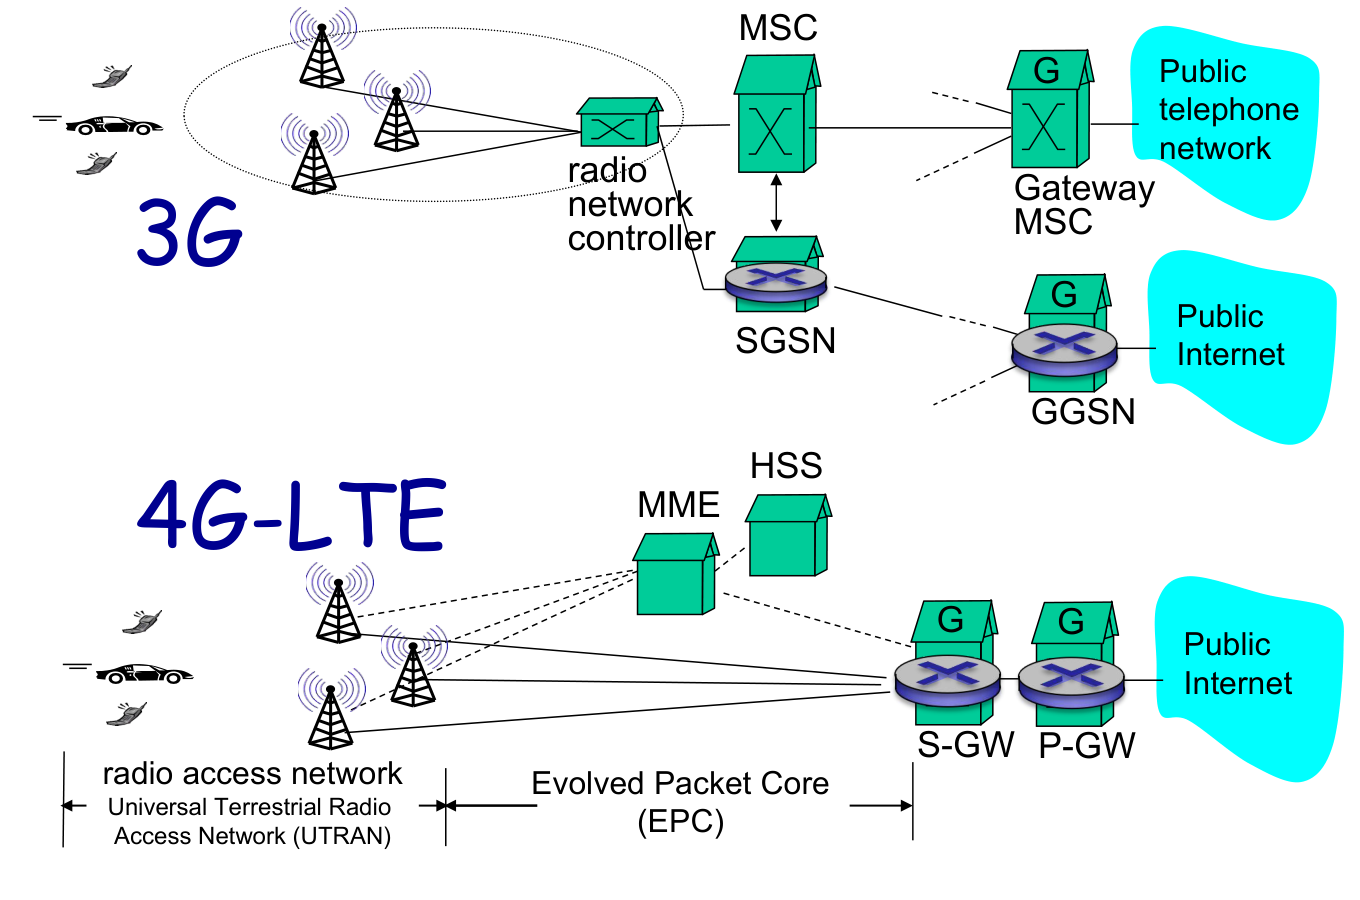
\includegraphics[width=.92\textwidth]{ch07-cellular-generations.png}\caption{课件中的 3G 与 4G LTE 网络结构对比：图中从无线接入网到核心网再到外部网络的连接关系不同。来源：\texttt{Chapter7-无线与移动网络.pdf}，PDF阅读器第45页（显示页45），局部截取。}\label{fig:ch07-cellular-generations}\end{figure}

\begin{figure}[H]\centering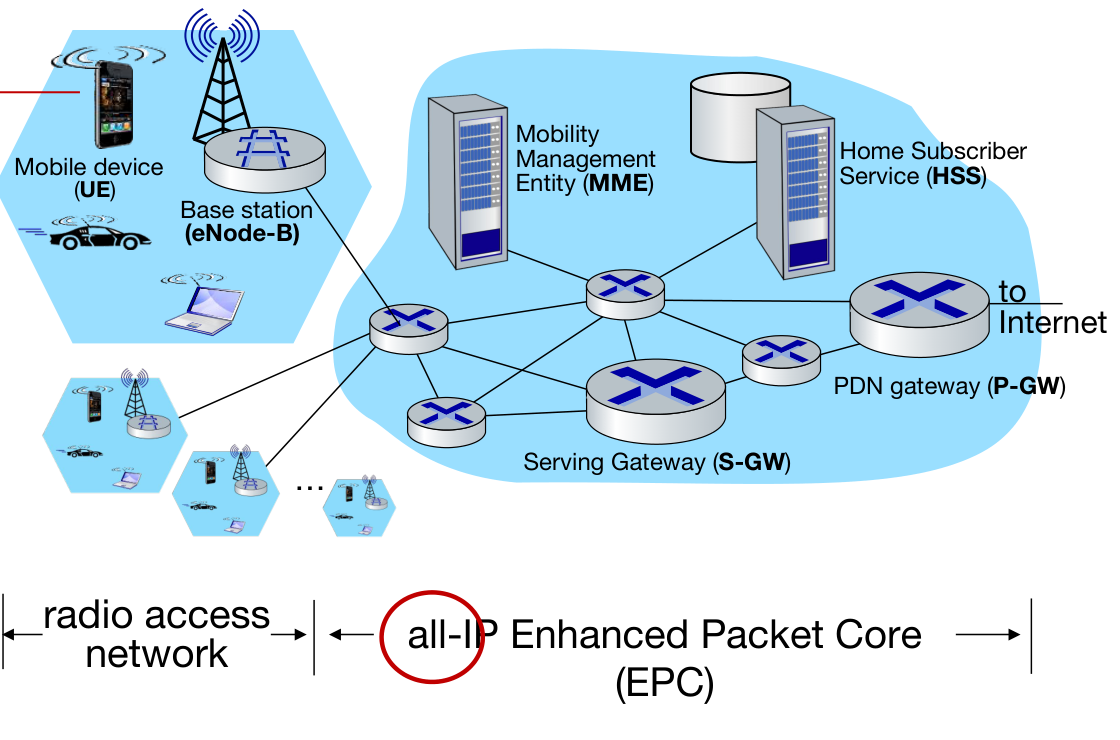
\includegraphics[width=.96\textwidth]{ch07-lte-architecture.png}\caption{LTE结构示意：左侧是 UE 与 eNode-B 无线接入，右侧 EPC 中的 MME/HSS 处理控制信息，S-GW/P-GW 转发用户数据。来源：\texttt{Chapter7-无线与移动网络.pdf}，PDF阅读器第49页（显示页49），局部截取。}\label{fig:ch07-lte-architecture}\end{figure}

课件列出的 LTE 部件职责可用“控制与数据分开”理解：MME 通过基站与移动设备通信，并向归属 HSS 查询鉴权、加密和服务信息；S-GW/P-GW 转发用户数据并建立隧道；基站管理本小区无线资源及终端。SIM（Subscriber Identity Module，用户识别模块）卡中保存 IMSI（International Mobile Subscriber Identity，国际移动用户识别码），用于标识用户及其归属网络，不等同于本次无线链路上的 MAC 地址或当前 IP 地址。课件第49、51页把 HSS 写作“Home Subscriber Service”，第90页写作“Home Subscriber Server”；本节采用课件第90页给出的 Server 写法。

\subsection{LTE 的数据面、协议栈与隧道}
在 LTE 首跳，课件从终端到基站列出分组数据汇聚（Packet Data Convergence）、无线链路控制 RLC（Radio Link Control）、媒体访问控制 MAC（Medium Access Control）和物理层等链路协议。分组数据汇聚层可做首部压缩与加密；RLC 可分片/重组并提供可靠数据传输；MAC 申请并使用无线时隙。下行采用频分复用 FDM（Frequency Division Multiplexing）并在频率信道内时分复用 TDM（Time Division Multiplexing），课件以 OFDM 说明子载波的正交性；课件图示每个活跃终端可分到两个或更多0.5 ms时隙、跨多个频率信道调度。调度算法由运营商实现，课件据此说明每终端可达到数百 Mb/s。

核心网广泛使用\textbf{隧道}：把终端的原始 IP 数据报放进 GTP-U（GPRS Tunneling Protocol User plane，用户面隧道协议）报文，再放入用户数据报协议（UDP，User Datagram Protocol）和外层 IP 数据报中，送到 S-GW；S-GW 解封装或重新封装后继续送往 P-GW。外层 IP 地址用于把隧道报文送到隧道另一端；内层 IP 数据报仍是终端与互联网服务器之间的原始数据。终端切换基站时，网络可更新隧道端点，而不要求每个外部通信对端都改写其目的地址。

\begin{figure}[H]\centering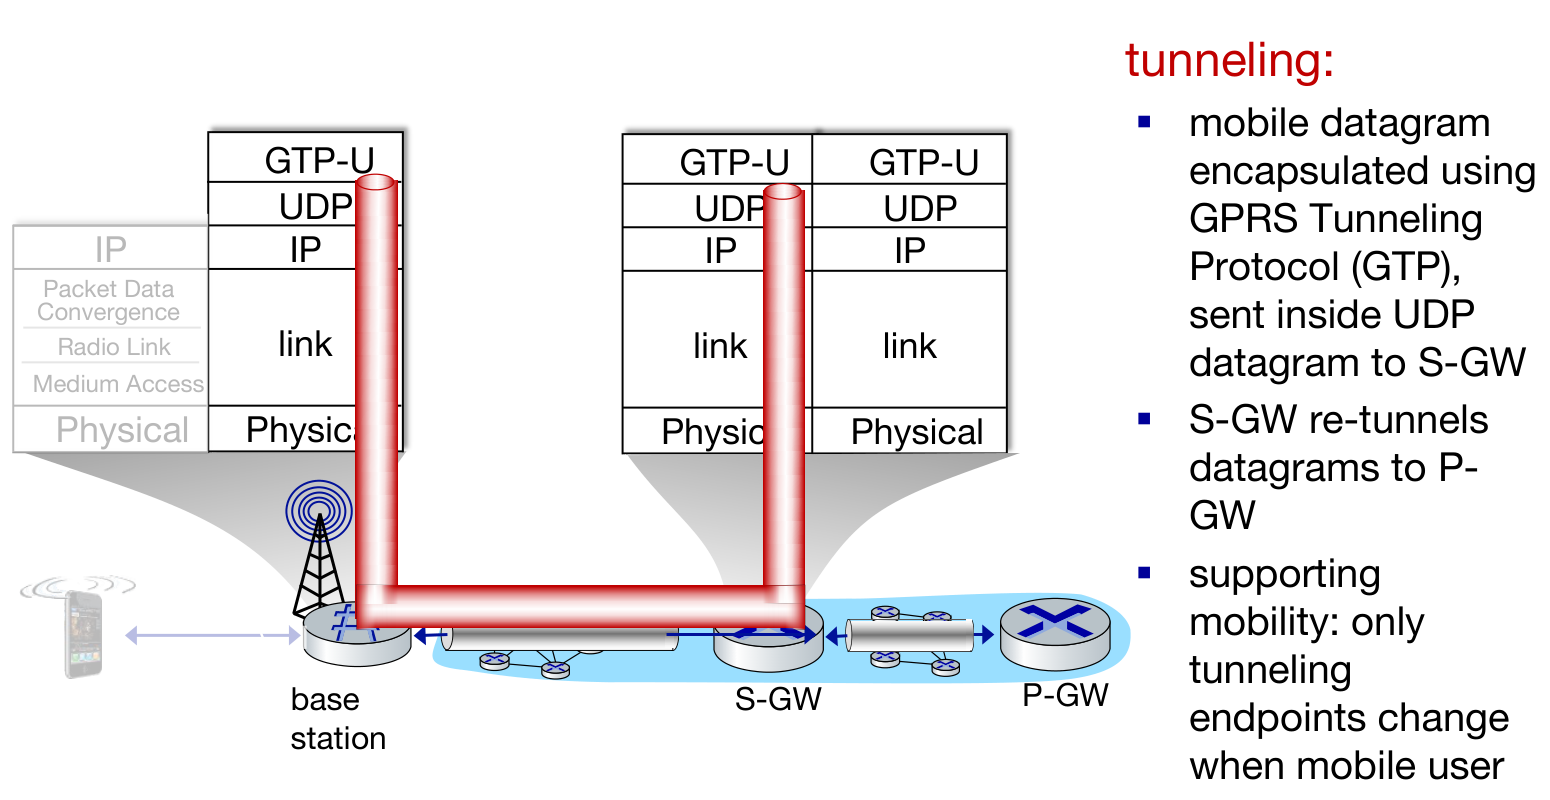
\includegraphics[width=.9\textwidth]{ch07-lte-tunnel-stack.png}\caption{LTE核心网隧道封装：红色路径表示终端数据经基站、S-GW到P-GW；右侧协议栈显示GTP-U/UDP/IP等外层封装。来源：\texttt{Chapter7-无线与移动网络.pdf}，PDF阅读器第57页（显示页57），局部截取。}\label{fig:ch07-lte-tunnel-stack}\end{figure}

移动设备与基站建立关联也有步骤：课件称基站每5 ms周期发送同步信号，设备先找到主同步信号，再找到该频率上的第二同步信号，读取带宽、网络配置和运营商信息；设备选择基站后仍要进行身份认证、状态配置及数据路径建立。休眠中的终端可以进入轻睡眠（课件举例为数百毫秒不活动后进入，并周期醒来检查下行帧）；无活动数秒后进入深睡眠，若休眠中移动到另一小区，醒来后需要重新建立关联。课件说明全球蜂窝网络通过运营商之间的互联点及公共互联网连接，归属 HSS 保存用户身份与服务信息；漫游时访问网络要能联系其归属网络。

\subsection{5G 课件概览}
课件以 5G NR（New Radio，新空口）说明后续发展：相对4G，课件列出的设计目标为峰值比特率提高10倍、时延降低10倍、流量容量提高100倍；频率范围 FR1（Frequency Range 1）约450 MHz--6 GHz、FR2（Frequency Range 2）约24--52 GHz。毫米波可支持更高数据率但覆盖距离较短，为此需要部署更密集的基站和更小的小区（课件称 pico-cell）。这些频段与目标倍数是课件中的技术概览，不是对每个实际部署的保证值。
\annotationarea[4]
\small 来源：课件PDF阅读器第40--61页（显示页40--61）；无线空口共享与无线介质可参考教材第2章§2.2.1，PDF第54--55页（印刷第43--44页）。教材未按课件展开2G/3G/4G/5G蜂窝核心网、LTE控制面和GTP隧道，本节相应机制以课件为依据。\normalsize

\section{网络移动管理基本原理}
\subsection{移动性的范围与位置管理}
从网络角度看，移动程度可以从低到高：设备完全不移动；设备在移动时关机，到新网络后再启动；设备在同一提供商网络内换接入点；设备在多个提供商网络间移动，同时保持正在进行的连接。课件重点讨论后两类：通信持续期间接入点或服务网络改变时，网络怎样知道设备当前位置并将数据送到那里。

一种办法是让互联网路由器通过常规路由信息广播移动节点的永久地址或编号所在位置，照普通前缀路由转发。课件认为这种办法理论上可行，但若为大量移动设备频繁发布主机级路由，会令全球路由表难以扩展。另一办法把功能放到网络边缘：设备或其归属网络登记当前接入位置，通信对端通过归属网络找到设备。

\textbf{归属网络}是用户订阅服务的运营商网络，保存用户身份、服务资料和当前所在位置；4G课件中这类资料由 HSS 保存。\textbf{访问网络}（visited network）是设备当前接入的其他运营商网络，双方通常需有漫游服务协议。在普通 ISP/Wi-Fi 接入中，往往没有统一的全球“归属网”登记机制，凭据可能是本地用户名、密码；因此不同 Wi-Fi 网络可能需要不同认证信息。

\subsection{间接路由与直接路由}
\textbf{间接路由}让通信对端始终向设备的永久地址发送。归属网络收到数据后查询设备最新登记的位置，再通过隧道把数据转发到访问网络；访问网络交付给设备。回复流量可以先回归属网络，也可以从访问网络直接发给通信对端。这样对端不必知道设备在哪个访问网络，移动到另一访问网后只需重新登记；代价是可能绕远，若通信双方本就在同一访问网络而数据仍经归属网，就形成“三角路由”式的低效路径。

\textbf{直接路由}由通信对端先向归属网络查询当前位置，再直接向访问网络发送数据。它能减少绕路，但对端必须得到并更新设备的访问地址；设备再次移动时，位置变化处理更复杂，通信也不再对端完全透明。

\begin{figure}[H]\centering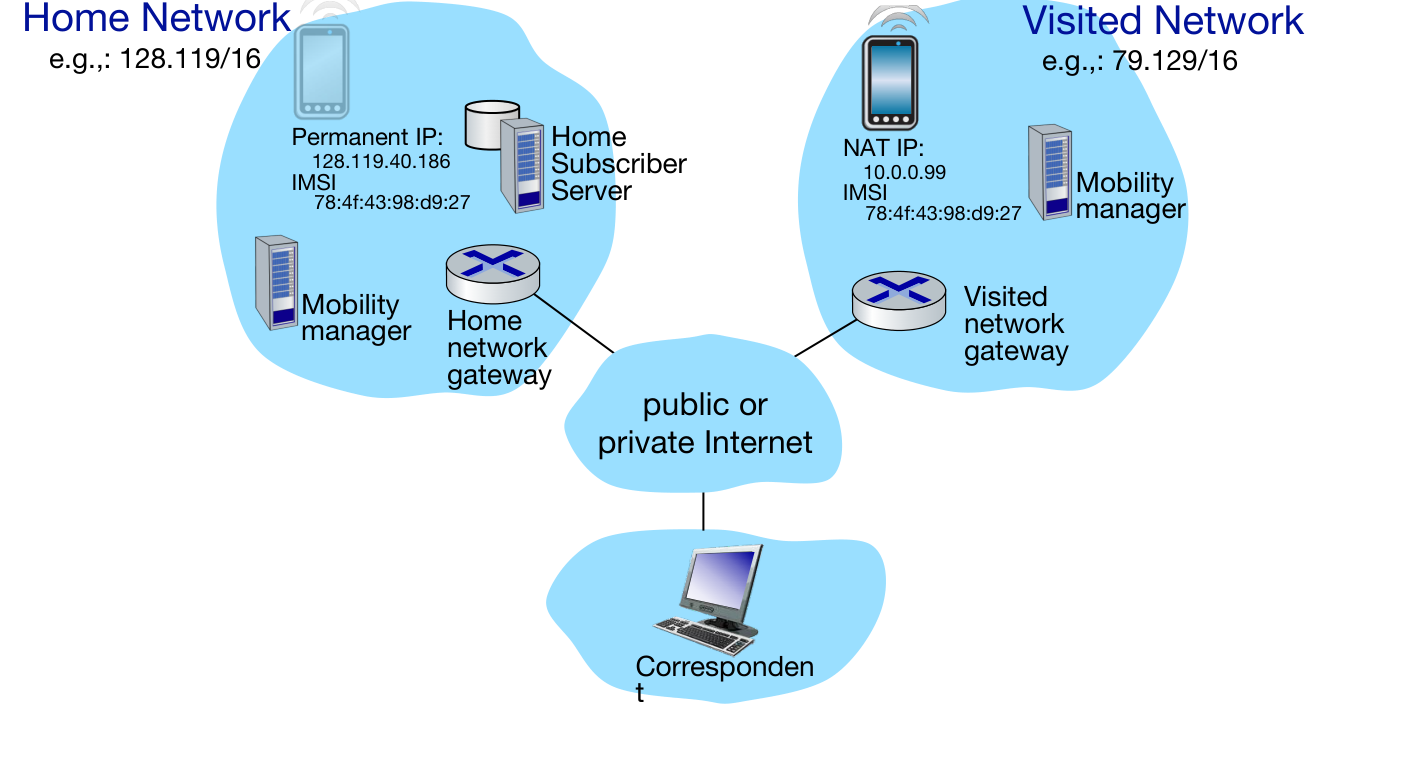
\includegraphics[width=.95\textwidth]{ch07-indirect-routing.png}\caption{归属网与访问网的拓扑关系：左右蓝色区域分别表示归属网络和访问网络，中间区域表示公共或专用互联网，下方区域表示通信对端；图中网关连线表示这些网络之间的互联关系。来源：\texttt{Chapter7-无线与移动网络.pdf}，PDF阅读器第69页（显示页69），局部截取。}\label{fig:ch07-indirect-routing}\end{figure}

在课件的 4G/5G 场景，移动设备先与访问网络基站关联并用 IMSI 表明归属；MME 与归属 HSS 配置控制面状态，确认设备当前位于访问网；MME 再设置用户面隧道，从归属 P-GW 经访问网转发到移动设备。设备换基站时，网络发起切换并更新转发端点。这样控制面负责“身份、位置与通道配置”，数据面负责“实际分组转发”。
\annotationarea[4]
\small 来源：课件PDF阅读器第63--74页（显示页63--74），第89--93页（显示页89--93）；移动IP与间接路由参考教材第4章§4.6，PDF第223--225页（印刷第212--214页）。教材未覆盖课件的蜂窝 HSS/MME 控制面分工。\normalsize

\section{移动 IP}
\subsection{永久地址、转交地址与代理}
移动 IP 是课件介绍的网络层移动性机制：移动节点离开归属网络后仍保留\textbf{永久地址}（归属地址），让通信对端继续使用同一目的地址；网络另为它登记当前访问位置，并把到达永久地址的数据转发过去。移动 IP 课件描述的是经归属网络间接转发的模型。

关键实体有：\textbf{移动节点}（mobile node），持有永久地址的移动设备；\textbf{归属代理}（home agent），位于归属网络，记录永久地址到当前转交地址的对应关系并截获发往移动节点的分组；\textbf{外地代理}（foreign agent），位于访问网络，协助移动节点登记和接收转发分组；\textbf{转交地址}（care-of address, COA），表示节点在访问网络中的当前可达位置。永久地址保持不变，转交地址随访问网络变化。

\subsection{代理发现、注册与数据转发}
课件把移动 IP 归纳为三项机制：间接路由、代理发现、向归属代理注册。代理发现时，归属代理或外地代理广播 ICMP（Internet Control Message Protocol，网际控制报文协议）代理通告；课件图中以 ICMP Router Advertisement（类型字段为9）及移动代理扩展表示，扩展携带代理类型标志、注册期限和一个或多个 COA。移动节点据此判断当前网络是否为归属网，或发现外地代理提供的转交地址。

移动节点获得 COA 后发起注册：注册请求携带移动节点永久地址、归属代理地址、COA、请求有效期和标识；外地代理把请求转给归属代理。归属代理接受后返回注册应答，外地代理再转给移动节点。归属代理据此保存绑定，知道“发往永久地址的分组应经隧道送到哪个 COA”。\textbf{参考书补充：}移动节点回到归属网络时，可注销或更新该绑定，恢复本地直接交付。

数据到达时，通信对端仍把永久地址作为目的 IP。归属代理收到后，在原数据报外再加一个新的 IP 首部，使外层目的地址为 COA；这是\textbf{隧道封装}，也叫“分组中的分组”。外地代理接收外层分组、移除外层首部，取出原始数据报后交给移动节点。外发数据则可由移动节点直接经过访问网络发往通信对端，因此去程经过归属代理、回程可能不经过它。

\begin{figure}[H]\centering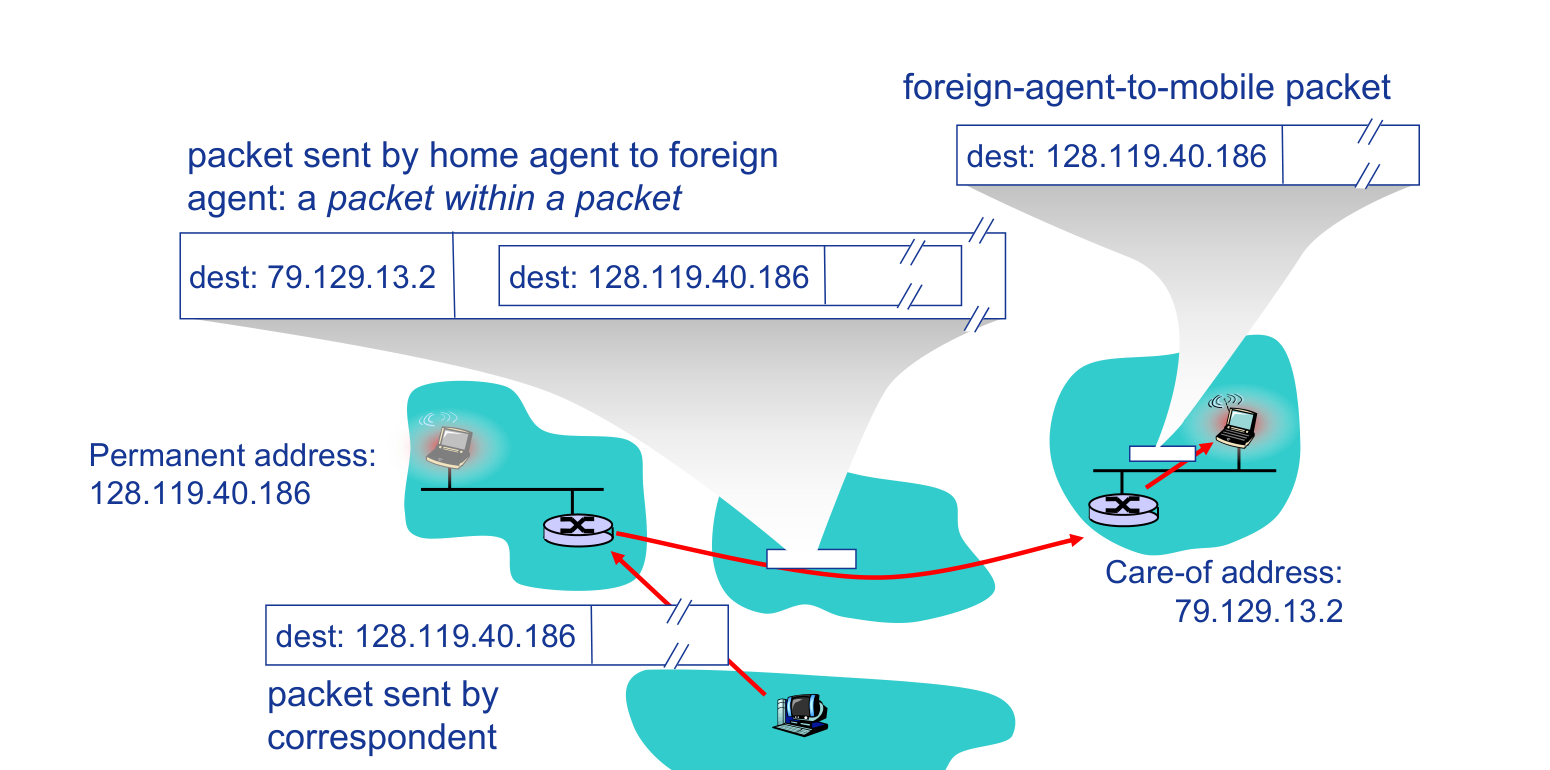
\includegraphics[width=.94\textwidth]{ch07-mobileip-tunnel.png}\caption{移动 IP 间接转发：原始分组目的地址是永久地址；归属代理封装后以 COA 为外层目的地址，经隧道送至外地代理；解封装后仍交给永久地址对应的移动节点。来源：\texttt{Chapter7-无线与移动网络.pdf}，PDF阅读器第78页（显示页78），局部截取。}\label{fig:ch07-mobileip-tunnel}\end{figure}

\textbf{课件注册示例（PDF第80页）：}访问网络为 79.129.13/24；移动节点永久地址为 128.119.40.186，外地代理提供 COA 79.129.13.2，归属代理地址为 128.119.40.7。节点发现代理后，请求把 79.129.13.2 登记到 128.119.40.7；请求示例中的 Lifetime（有效期）为9999，标识号为714；返回应答使用相同标识号，示例同意的有效期为4999。归属代理收到并接受登记后，便可把送往 128.119.40.186 的分组经隧道发往 79.129.13.2。课件给出的有效期数值是报文示例，重点是请求与应答的往返登记关系。

\begin{figure}[H]\centering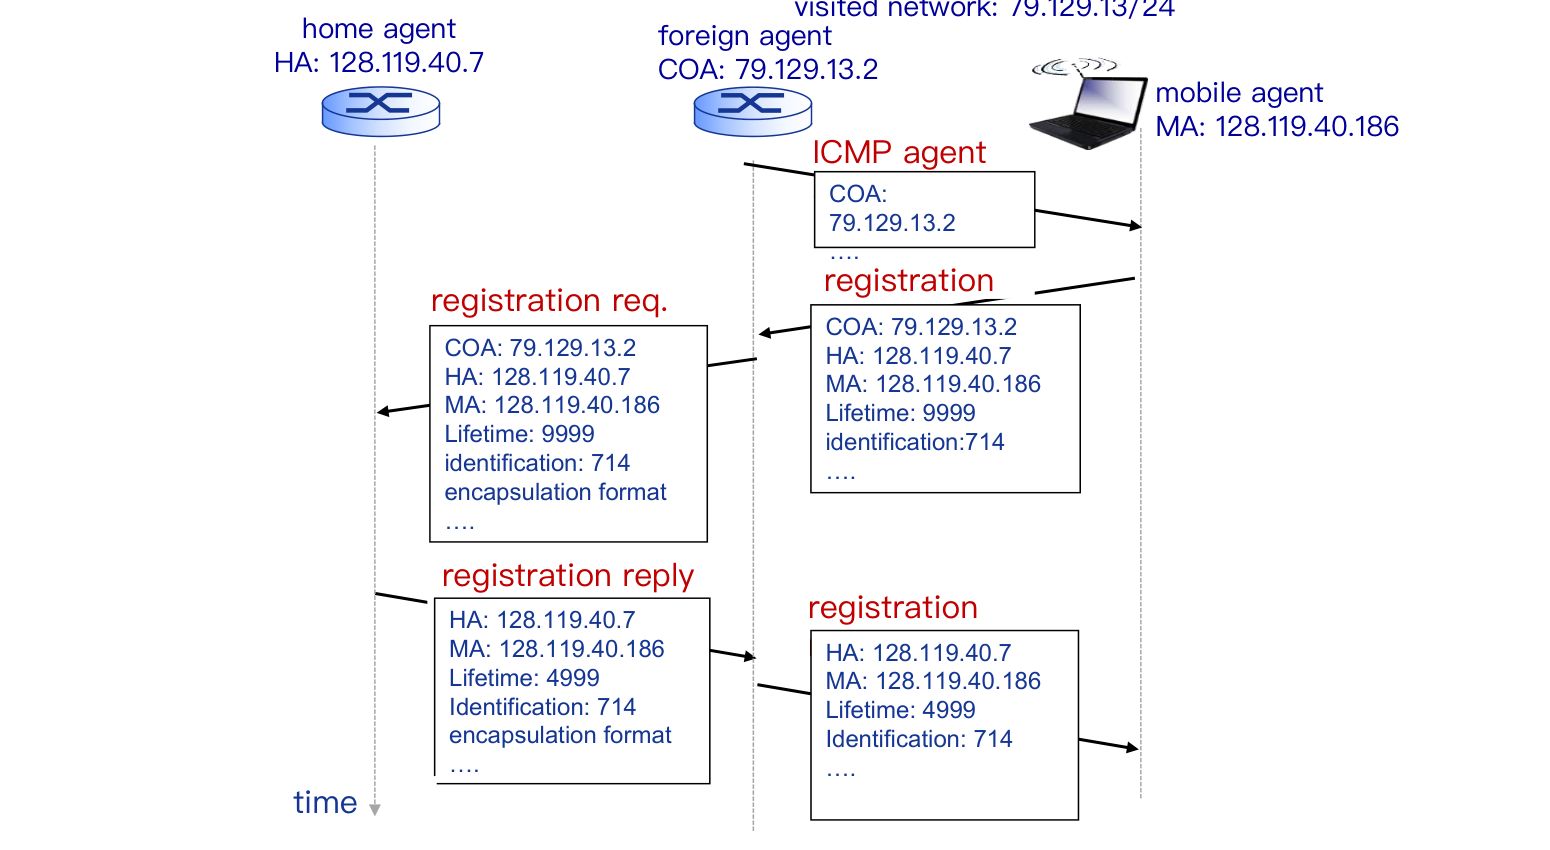
\includegraphics[width=.91\textwidth]{ch07-mobileip-registration.png}\caption{移动 IP 注册时间线：代理先通告 COA，移动节点请求登记到归属代理，注册应答沿外地代理返回；数值字段是课件中的示例。来源：\texttt{Chapter7-无线与移动网络.pdf}，PDF阅读器第80页（显示页80），局部截取。}\label{fig:ch07-mobileip-registration}\end{figure}

\textbf{间接与直接路由比较。} 间接路由把位置管理集中在归属代理，通信对端仍只需知道永久地址，移动后便于维持连接，但可能绕路。直接路由要求通信对端查询移动节点的访问地址并直接发送，较少绕路，却要把位置变化告知通信对端。课件指出早期移动 IP 采用隧道间接路由；教材也强调归属地址不变、COA动态变化及归属代理到外地网络的隧道。

\textbf{教材补充练习（移动 IP，参考书PDF第224--225页）：}
\begin{enumerate}[nosep]
  \item 判断“移动节点到达新网络后，把新的可达信息通知外地代理”是否正确。\textbf{解：}不正确。移动节点把 COA 等登记信息交给外地代理协助转发；真正需要获知该移动节点新位置并建立转发绑定的是归属代理。归属代理随后把分组隧道到该 COA。
  \item 移动 IP 的归属地址和转交地址如何变化？\textbf{解：}归属地址对应归属网络，移动时保持不变；COA 标识访问网中的当前可达位置，换访问网络时会改变，返回归属网时可注销。
  \item 主机 160.80.40.20/16 移动到不属于 160.80/16 的网络，若没有移动 IP，能否收发？\textbf{解：}它可把原永久地址作为源地址发出分组，访问网络的默认路由仍可能转发出站流量；但发往 160.80.40.20 的入站分组会被路由到其归属前缀，而不会自然到达新网络。因此在课件所问的直接收发中，能直接发送、不能直接接收（对应教材选项D）。
\end{enumerate}
\annotationarea[4]
\small 来源：课件PDF阅读器第76--80页（显示页76--80）；参考教材第4章§4.6.1--§4.6.4，PDF第223--225页（印刷第212--214页）。课件第76页列RFC 5944，第77页列RFC 3344，引用版本不同；本文按课件给出的移动IP基本模型整理，不据此扩展协议版本差异。\normalsize

\section{移动通信网络的移动管理}
\subsection{GSM 归属/访问位置登记与寻呼路由}
课件用 GSM（Global System for Mobile Communications，全球移动通信系统）说明蜂窝语音网络中的位置登记。\textbf{归属位置寄存器} HLR（Home Location Register）位于归属网络，保存用户永久电话号码、服务资料及当前所在网络等信息；\textbf{访问位置寄存器} VLR（Visitor Location Register）为当前访问网络中的用户保存临时登记信息。访问网络可以就是归属网络。

当呼叫者拨打移动用户号码时，呼叫先到归属网络 MSC；归属 MSC 查询 HLR，得到该用户当前访问网络的可路由号码，再建立通往访问网络 MSC 的第二段呼叫；访问 MSC 最后通过相应基站连接移动用户。关键点是电话网络先联系用户归属地，再由归属位置记录找到当前访问网络。

\subsection{GSM 切换}
\textbf{切换}是通信中的移动设备从旧基站转到新基站，同时尽量保持当前通话或连接。课件列出的触发理由包括：新基站信号更强、持续连接更可靠/节省电池，或网络需要负载均衡。GSM 规范描述如何进行切换，但不强制网络必须按哪一种策略决定何时切换。

同一 MSC 管理范围内的切换按课件时序可读成八步：
\begin{enumerate}[nosep]
  \item 旧基站向 MSC 报告即将切换，并提供一个或多个候选新基站。
  \item MSC 为到新基站的路径分配资源。
  \item 新基站为移动设备预留无线信道。
  \item 新基站通知 MSC 和旧基站“新信道准备好”。
  \item 旧基站通知移动设备切换到新基站。
  \item 移动设备和新基站激活新信道。
  \item 移动设备通过新基站向 MSC 报告切换完成，MSC 改走新路径。
  \item 释放 MSC 与旧基站之间不再需要的资源。
\end{enumerate}

\begin{figure}[H]\centering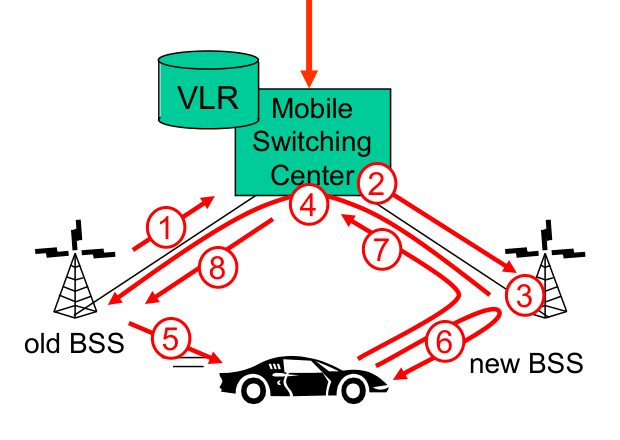
\includegraphics[width=.9\textwidth]{ch07-gsm-handoff.png}\caption{同一 MSC 内 GSM 切换的八个事件：旧基站启动流程，新基站先准备信道，移动设备接入新基站后 MSC 改路并释放旧资源。红色数字表示事件顺序。来源：\texttt{Chapter7-无线与移动网络.pdf}，PDF阅读器第85页（显示页85），局部截取。}\label{fig:ch07-gsm-handoff}\end{figure}

若设备在通话中切换到另一个 MSC，课件把最初接入的 MSC 称为\textbf{锚 MSC}（anchor MSC）。通话仍经锚 MSC；每次移动到新 MSC 时，可在原转发链上增加新的 MSC。这样可以继续保持通话，但链路可能越来越长；网络可选做路径最小化以缩短转发链。

\subsection{4G LTE 基站切换}
LTE 中 MME 管理移动状态，S-GW/P-GW 处于数据路径上。课件把基站间切换分为控制信令和转发调整两部分。以下按 PDF 第92--93页逐事件解释：
\begin{enumerate}[nosep]
  \item 源基站选择目标基站，发送 Handover Request（切换请求）。
  \item 目标基站预分配无线时隙/资源，并向源基站发送 Handover Request Acknowledgment（切换请求确认），其中包含供移动设备使用的信息。
  \item 源基站把目标基站信息通知移动设备；移动设备开始通过目标基站通信。
  \item 源基站停止向移动设备直接发送数据，而把暂时到达的分组转发给目标基站，由目标基站通过无线链路交付。
  \item 目标基站告知 MME 自己成为该移动设备的新基站；MME 指示 S-GW 更新隧道端点。
  \item 目标基站向源基站确认切换结束，源基站释放旧资源。
  \item 移动设备数据改走从目标基站到 S-GW 的新隧道。
\end{enumerate}

\begin{figure}[H]\centering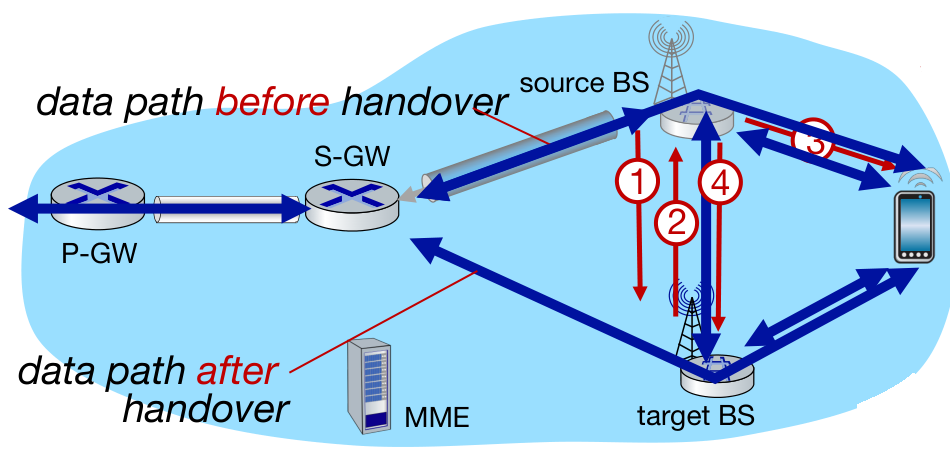
\includegraphics[width=.96\textwidth]{ch07-lte-handover-1.png}\caption{LTE 基站切换前半段：源基站请求目标基站准备，目标分配无线资源，移动设备改由目标基站接入，源基站临时转发尚未送达的分组。来源：\texttt{Chapter7-无线与移动网络.pdf}，PDF阅读器第92页（显示页92），局部截取。}\label{fig:ch07-lte-handover-1}\end{figure}
\begin{figure}[H]\centering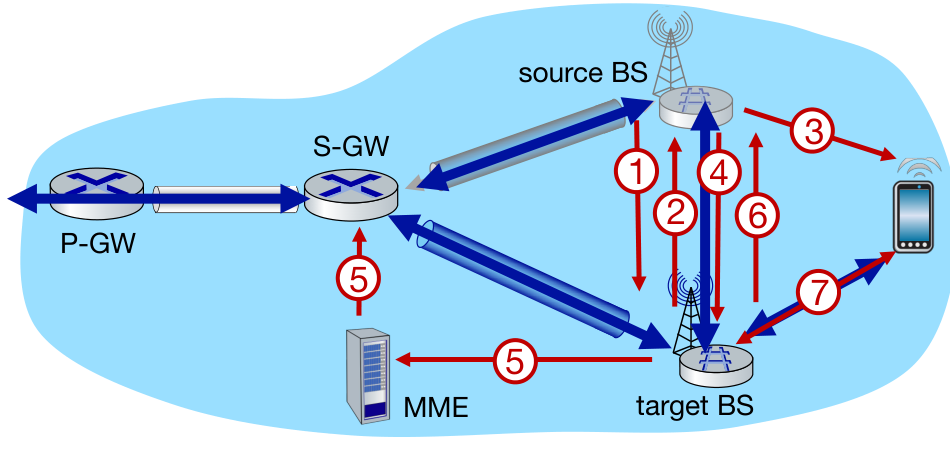
\includegraphics[width=.94\textwidth]{ch07-lte-handover-2.png}\caption{LTE 基站切换后半段：目标基站更新 MME，MME 改设 S-GW 隧道端点，确认后释放源基站资源，数据最终经目标基站的新隧道转发。来源：\texttt{Chapter7-无线与移动网络.pdf}，PDF阅读器第93页（显示页93），局部截取。}\label{fig:ch07-lte-handover-2}\end{figure}

\subsection{蜂窝移动管理与移动 IP 的联系}
课件用比较表把 GSM 组件与移动 IP 概念对应：归属系统类似归属网络；归属 MSC/HLR 的职责与归属代理部分相似；访问 MSC/VLR 的职责与外地代理部分相似；GSM 的移动台漫游号码 MSRN（Mobile Station Roaming Number）承担访问路径的可路由地址作用，移动 IP 中相应概念是 COA。二者都需要归属侧位置记录，并把发往永久身份/地址的数据转到当前访问位置；但一个是蜂窝电话呼叫架构，一个是 IP 数据报转发架构，组件名称和协议流程不能直接等同。

\annotationarea[4]
\small 来源：课件PDF阅读器第82--93页（显示页82--93）；移动 IP 与 GSM 对照参考教材第4章§4.6，PDF第223--225页（印刷第212--214页）。GSM、LTE 的 HLR/VLR、MSC、MME 与切换细节以课件为依据。\normalsize

\section{无线与移动对高层协议的影响}
无线链路和移动接入不会改变网络层的尽力而为服务模型：传输控制协议（TCP，Transmission Control Protocol）、用户数据报协议（UDP，User Datagram Protocol）和 IP 仍可运行在无线网络上。变化主要出现在性能方面：无线误码会使链路层丢弃数据或通过重传带来额外时延；切换过程中也可能短暂丢包或延迟。TCP 看到丢包时通常把它当成拥塞信号，缩小拥塞窗口；但无线链路的位错误或切换丢包未必来自网络拥塞，因此可能不必要地降低吞吐量。实时业务会感受到额外时延，而无线频谱/带宽本身也是稀缺资源，需要合理共享。

\textbf{复习时抓住因果链：} 无线误码、隐藏终端和切换都可能引起丢包/等待；链路层的确认、重传和调度可改善链路可靠性，但会增加时延；传输层和应用层观察到的是最终时延与丢失，未必知道其来自拥塞、无线误码还是移动切换。
\annotationarea[4]
\small 来源：课件PDF阅读器第95页（显示页95）。本节具体性能影响依课件总结；参考教材相应章节用于核对无线链路、可靠传输与TCP拥塞反应，不将教材未在此处展开的机制写成课件结论。\normalsize
